%! TEX program = xelatex
%! TEX root = main.tex
%! TEX program = xelatex
%! TEX root = main.tex
\documentclass[a4paper,11pt]{article}
\usepackage{geometry}
\geometry{left=1.5cm,right=5mm,top=1cm,bottom=1.5cm}
%============================中文支持==============================
%中文自动换行
\XeTeXlinebreaklocale "zh"
\XeTeXlinebreakskip = 0pt plus 1pt
%中文编码支持
\usepackage{xltxtra,fontspec,xunicode}
 %中文支持包
\usepackage{xeCJK}
%书签
\usepackage{CJKutf8}
%1. 文件开头加入\usepackage{pdfpages}
%2. 文件中使用\includepdf{mypdffile.pdf} 插入pdf文件。
\usepackage{pdfpages}
%============================图形以及符号===============================
%避免浮动
\usepackage{float}
%插入图片的宏包
\usepackage{graphicx}
%图标包 typicous
\usepackage{typicons}
%作图
\usepackage{tikz}
\usetikzlibrary{graphs}
\usepackage{pgfplots}
\usepackage{mathtools}
\usepgfplotslibrary{groupplots}
%=======================页面,段落,行距,超链接设置===============================
\usepackage{ulem}  %下划线(uline),波浪线(uwave),双下划线(uuline)
                   %删除线(sout),斜删除线(xout),虚线(dashuline),加点(dotuline)
\usepackage{geometry} %横向布局,用横向布局时,使用\usepackage[landscape]{geometry}
%\usepackage[a3paper]{geometry} %a3纸张大小
%\geometry{left=1cm,right=1cm,top=1.5cm,bottom=1.5cm}
\usepackage{indentfirst} %缩进
%%设置缩进
\setlength{\parindent}{2em}
%设置行距
\linespread{1.6}
%加入超链接,用法为\url{https://www.google.com}或\href{https://www.google.com}{Google}
%这里还必须指定为unicode方式,以使书签正常显示
\usepackage[unicode,colorlinks,linkcolor=black,anchorcolor=blue,citecolor=green]{hyperref}
%========================数学公式==================================
\usepackage{latexsym}
\usepackage{amsmath}                 % AMS LaTeX宏包
\usepackage{amssymb}                 % 用来排版漂亮的数学公式
\usepackage{amsbsy}
\usepackage{amsthm}
\usepackage{amsfonts}
\usepackage{mathrsfs}                % 英文花体字体
\usepackage{bm}                      % 数学公式中的黑斜体
\usepackage{relsize}                 % 调整公式字体大小:\mathsmaller, \mathlarger
\usepackage{caption}                % 浮动图形和表格标题样式
\usepackage{times}
\usepackage{esint} %面积分符号\oiint
\usepackage{mathdots}
\allowdisplaybreaks
%========================字体设置=================================
%中文字体
\setCJKmainfont{YouYuan}
\setCJKsansfont{YaHei Consolas Hybrid}
\setCJKmonofont{YaHei Consolas Hybrid}
\setCJKfamilyfont{SimSun}{SimSun}
\setCJKfamilyfont{SimHei}{SimHei}
\setCJKfamilyfont{FangSong}{FangSong}
\setCJKfamilyfont{KaiTi}{KaiTi}
\setCJKfamilyfont{YouYuan}{YouYuan}
\newcommand{\song}{\CJKfamily{SimSun}} % 宋体
\newcommand{\hei}{\CJKfamily{SimHei}}   % 黑体
\newcommand{\fs}{\CJKfamily{FangSong}}     % 仿宋
\newcommand{\kai}{\CJKfamily{KaiTi}}   % 楷体
\newcommand{\yy}{\CJKfamily{YouYuan}}   % 楷体
%英文字体
\setmainfont{Source Code Pro}
\setmonofont{Source Code Pro}
% 其他英文字体别名
% 使用方法如下:{\sp :g/pattern/s/old/new/g}
\newfontfamily\sp{Segoe Print}

%数学长等号
\usepackage{extarrows}
%特殊符号
\usepackage{bbding}
%矩阵中使用虚线的宏包
\usepackage{pmat}
%=======================页眉页脚设置=======================
%以下两行设置脚注
\renewcommand*{\thefootnote}{\arabic{footnote}} %脚注为罗马数字编号
\usepackage[perpage,stable]{footmisc} % 每页重新编号,如果不希望这样可以去掉 [perpage]

\usepackage{fancyhdr}
\usepackage{pageslts}
%设置subsubsection{}
%\setcounter{secnumdepth}{5}%设置标题深度为5
%subsubsection{} level3
%paragraph{} level4
%subparagraph{} level5
\pagenumbering{arabic} %默认选用的页码为数字格式
%==========================代码格式化包===============================
\usepackage{fancyvrb}
\usepackage{color}
\usepackage[colorlinks,linkcolor=black,anchorcolor=blue,citecolor=green]{hyperref}
\usepackage{listings}

%一般 lstlisitng 样式
\lstdefinestyle{general}{
    basicstyle=\linespread{0.8}\small\ttfamily, % 代码行距设置为 0.8
    frameround=fttt,
    frame=trBL,
    numbers=left,
    firstnumber=1,
    morecomment=[l],
    keepspaces=true,
    morecomment=[s][\color{blue}]{/*+}{*/},
    morecomment=[s][\color{green}]{/*-}{*/},
    morecomment=[s][\color{red}]{/**}{*/},
}

% 模拟 verb 环境实现自动换行
\lstdefinestyle{verb} {
    aboveskip=10pt, % lst 和上面的间距
    belowskip=0pt, % lst 和下面的间距
    basicstyle=\linespread{0.8}\small\ttfamily,  % 代码行距设置为 0.8
    columns=flexible,
    breaklines=true, % 启用自动换行
    frame=single, % 单边框
    postbreak=\mbox{\textcolor{red}{$\hookrightarrow$}\space}, % 换行符号
}

%自定义行间极限符号
\newcommand{\ilim}{\lim\limits}
%=========================自定义目录====================
\renewcommand{\abstractname}{}
\renewcommand{\contentsname}{目录}
\renewcommand{\refname}{参考文献}
\renewcommand{\today}{\number\year 年 \number\month 月 \number\day 日}
% 自定义图片标题的名称
\renewcommand{\figurename}{图}
% 自定义表格标题的名称
\renewcommand{\tablename}{表}
% 自定义代码段标题
\renewcommand{\lstlistingname}{代码}

%自定义向量粗体显示
\renewcommand{\vec}[1]{\boldsymbol{#1}}
%\usepackage{fouriernc}
%改善自定义圆圈数字
%在枚举环境中可以这么做:
%\begin{enumerate}[label=\protect\circled{\arabic*}]
%\item First item
%\item Second item
%\item Third item
%\item Fourth item
%\end{enumerate}
%在单个语句中可以这么做:\circled{1} \circled{2} \circled{3}
\usepackage{enumitem}
% 注意这种圆圈数字有限制,不能在 listing 环境中使用
% 在 listing 中可以使用\textcircled{\raisebox{-0.9pt}{8}}
\newcommand*\circled[1]{\tikz[baseline=(char.base)]{
            \node[shape=circle,draw,inner sep=2pt] (char) {#1};}}
%加载目录以及标题设置宏包
\usepackage{titlesec}
\usepackage{titletoc}
%设置目录中的字体,编号以及边距:
\titlecontents{part}[10mm]                          %设置part的编号距离纸张左侧10mm处开始打印
{\fontsize{13pt}{10pt}\selectfont \song}            %字体设置为12pt,行距设置为10pt,字体设置为宋体
{\contentslabel{2em} }                              %part编号和标题之间的距离为2em
{}
{ \contentsmargin{4mm} \titlerule*{.}\contentspage} %设置标题右侧页码与连接符号之间的距离为4mm,设置标题和页码之间的连接符号为点,并设置间隔距离


\renewcommand\thesection{\arabic{section}}          %解决section从0.x开始的问题
\titlecontents{section}[10mm]                       %设置section的编号距离纸张左侧10mm处开始打印
{\fontsize{12pt}{10pt}\selectfont \song}            %字体设置为12pt,行距设置为10pt,字体设置为宋体
{\contentslabel{2em} }                              %section编号和标题之间的距离为2em
{}
{ \contentsmargin{4mm} \titlerule*{.}\contentspage} %设置标题右侧页码与连接符号之间的距离为4mm,设置标题和页码之间的连接符号为点,并设置间隔距离


\titlecontents{subsection}[22mm]
{\fontsize{11pt}{10pt}\selectfont \song}
{\contentslabel{3em}}
{}
{ \contentsmargin{4mm} \titlerule*{.}\contentspage}

\titlecontents{subsubsection}[37mm]
{\fontsize{10pt}{10pt}\selectfont \song}
{\contentslabel{4em}}
{}
{ \contentsmargin{4mm} \titlerule*{.}\contentspage}
%%设置正文中的标题大小以及字体
\titleformat{\part} {\LARGE\yy} {\thesection}{1em}{\centering}{} %part标题居中显示
\titleformat{\section} {\LARGE\yy} {\thesection}{1em}{}
\titleformat{\subsection} {\Large\yy} {\thesubsection}{1em}{}
\titleformat{\subsubsection} {\large\yy} {\thesubsubsection}{1em}{}

%设置分类图
\newenvironment{subgroup} {$\left\{\tabular{l}} {\endtabular\right.$}
%\begin{subgroup}
%    数模混合计算机 \\[1em]
%    模拟计算机\\[1em]
%    数字计算机
%    \begin{subgroup}
%        专用计算机 \\
%        通用计算机
%        \begin{subgroup}
%            巨型机\\
%            大型机\\
%            小型机\\
%            微型机\\
%            工作站\\
%            服务器
%        \end{subgroup}
%    \end{subgroup} \\[5em]
%    未来计算机
%    \begin{subgroup}
%        量子计算机 \\
%        生物计算机
%    \end{subgroup}
%\end{subgroup}


\begin{document}
% preface for a notes
%%! TEX program = xelatex
%! TEX root = main.tex
\title{笔记}
\author{by bugnofree}
\date{2017-11-05 $\sim$ ???}
\maketitle
\vfill
\begin{center}
\scalebox{3.0}{$\int_{-\infty}^{+\infty} e^{-x^2}dx=\sqrt{\pi}$}
\end{center}
\vfill
\begin{flushright}
谨以此献给奋斗的那些岁月
\end{flushright}
\thispagestyle{empty}
\newpage

\tableofcontents


% preface for a sticky
%! TEX program = xelatex
%! TEX root = main.tex
\title{分布式存储系统 RLFS 的设计与实现 \\ \href{https://github.com/ikey4u/rlfs}{\small{https://github.com/ikey4u/rlfs}}}
\author{bugnofree}
\date{2018-09-14}
\maketitle
\tableofcontents


\section{背景}
\subsection{FUSE 系统架构}
FUSE 的全称是 Filesystem in user space, 即用户空间上的文件系统,
它给用户提供了一个软件接口, 使得用户可以在不编辑内核代码的情况下即可创建自己的文件系统,
其实现的主要原理是在用户空间运行用户的文件系统代码,
同时通过内核模块 FUSE 与实际的内核接口交互. FUSE 的基本原理图如 \ref{fig:fuse_structure}
所示.

\begin{figure}[H]
    \centerline{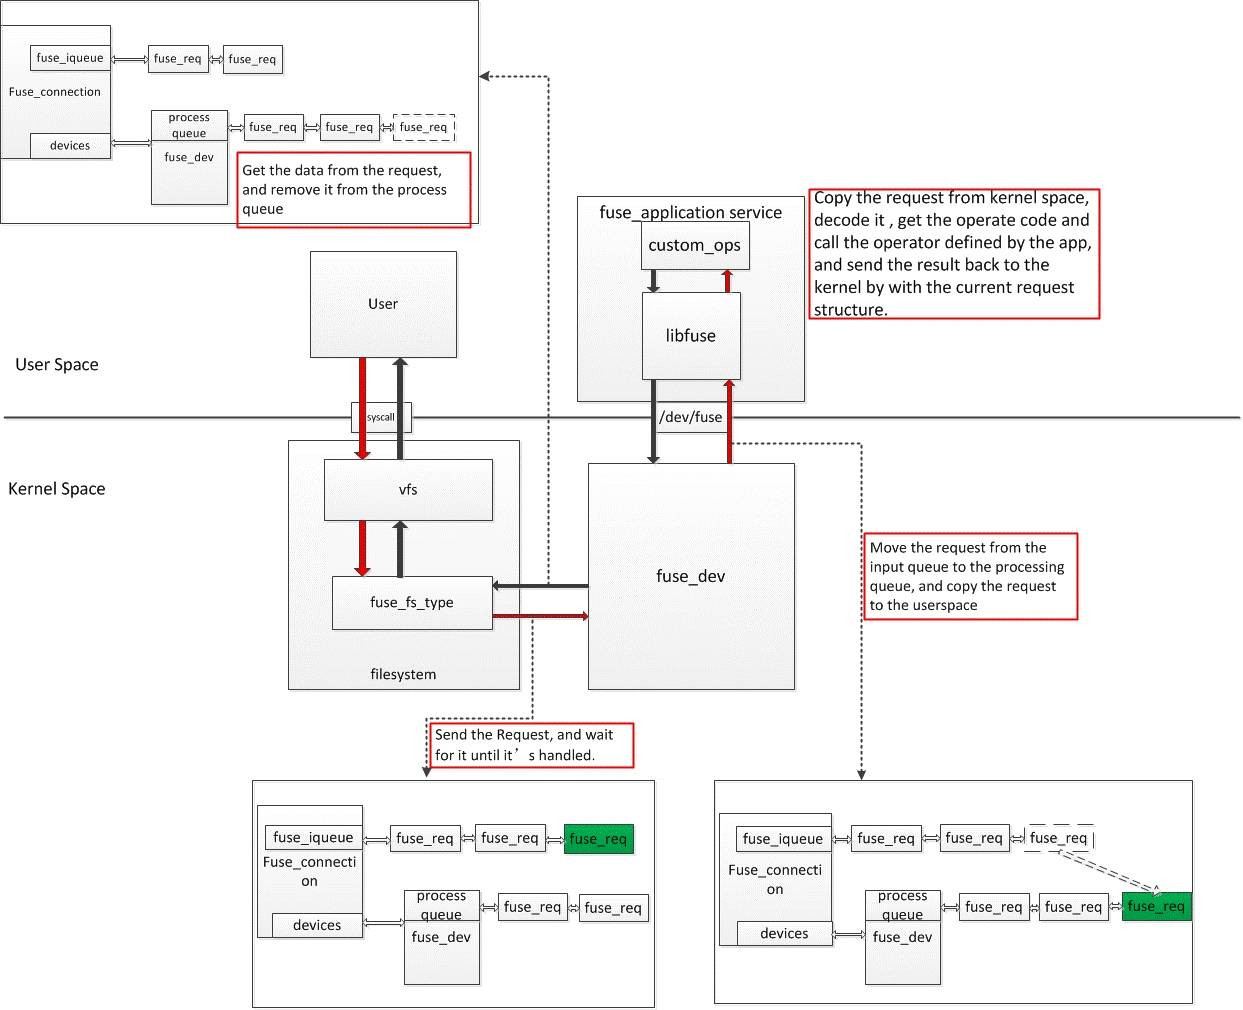
\includegraphics[width=0.8\textwidth]{./Figures/fusestruct.png}}
    \caption{FUSE 架构图}
    \label{fig:fuse_structure}
\end{figure}

当用户在挂载的目录上执行文件操作时, 用户空间的请求将被 VFS 模块截获,
并重定向到 FUSE 内核模块, FUSE 内核模块通过 /dev/fuse 文件与 libfuse 库进行通信,
然后 fuse 客户端(我们基于 libfuse 开发的程序)开始处理用户请求, 处理完之后将响应返回给内核,
内核再将响应显示给用户.

本文系统是基于 libfuse (2.9.7 版本) 开发的文件系统, 因此了解 libfuse 的架构十分必要.
libfuse 的工作流如图 \ref{fig:fuseflow} 所示.

\begin{figure}[H]
    \centerline{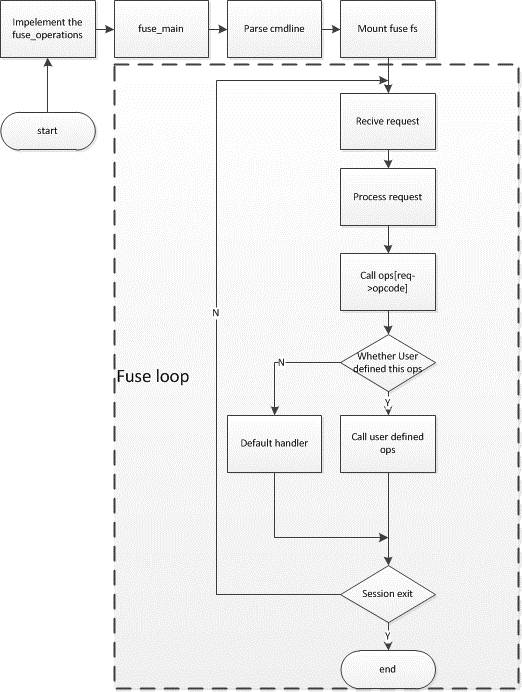
\includegraphics[width=0.8\textwidth]{./Figures/fuseflow.png}}
    \caption{libfuse 流程}
    \label{fig:fuseflow}
\end{figure}

在图 \ref{fig:fuseflow} 中可以看到, 我们需要实现 fuse 暴露给我们的接口,
这个接口实际上是一个结构体, 其名称为 \verb|fuse_operations|, 其定义如下

\begin{lstlisting}[style=verb]
struct fuse_operations {
int (*getattr) (const char *, struct stat *, struct fuse_file_info *fi);
int (*create) (const char *, mode_t, struct fuse_file_info *);
int (*open) (const char *, struct fuse_file_info *);
int (*read) (const char *, char *, size_t, off_t, struct fuse_file_info *);
int (*write) (const char *, const char *, size_t, off_t, struct fuse_file_info *);
int (*opendir) (const char *, struct fuse_file_info *);
int (*readdir) (const char *, void *, fuse_fill_dir_t, off_t, struct fuse_file_info *, enum fuse_readdir_flags);
// ...
}
\end{lstlisting}

我们需要实现相应的函数, 对该结构体进行填充即可, 实现的函数通常应该有一个前缀(但是不是必须的),
这里选取 rlfs, 比如实现 init 时的函数名就选取为 \verb|rlfs_init|.

当把函数实现完之后, 填充 \verb|fuse_operations| 结构体即可, 如下

\begin{lstlisting}[style=verb]
static struct fuse_operations rlfs_operations = {
    .init	= rlfs_init,
    .release = rlfs_release,
    // ...
};
\end{lstlisting}

之后便是在主函数中调用图 \ref{fig:fuseflow} 里面的 \verb|fuse_main| 函数, 如下
\begin{lstlisting}[style=verb]
int main(int argc, char** argv) {
	return fuse_main(argc, argv, &rlfs_operations, private_data);
}
\end{lstlisting}

其中 \verb|fuse_main| 函数共有四个参数, 其含义依次如下

\begin{itemize}
    \item argc, argv: 用户 mian 函数参数.
    \item \verb|rlfs_operations|: \verb|fuse_operations| 对象.
    \item \verb|private_data|: 用户私有数据结构体.
\end{itemize}

\subsection{FUSE 主要接口}

libfuse 暴露的接口很多, 有些是必要实现的, 而有些则不是. libfuse 中最重要的莫过于是
getattr 函数, 一个可用的文件系统必须首先实现该函数, 此函数的定义如下:

\begin{lstlisting}[style=verb]
int (*getattr) (const char *path, struct stat *stbuf);
\end{lstlisting}

这个函数的作用是用于获取文件属性, 文件的路径为 path, 是一个相对路径(相对于挂载点),
在 libfuse 提供的所有接口中, 除了 init(初始化文件系统) 和 destroy(在文件系统退出时调用, 可
以用于清理用户私有数据), 其他的大多数接口的第一个参数都是当前访问文件的相对路径.
假如说挂载目录是 \verb|~/point|, 那么访问该目录下面的 fuse.h 文件,
getattr 函数体内得到的 path 值将会是 \fbox{/fush.h}, 所以为了获取绝对路径值,
可以和挂载点拼接.

然后看第二个参数, 这是一个 linux 下的结构体 struct stat, 可以使用 \fbox{man stat} 来查看,
如图 \ref{fig:stat} 所示.

\begin{figure}[H]
    \centerline{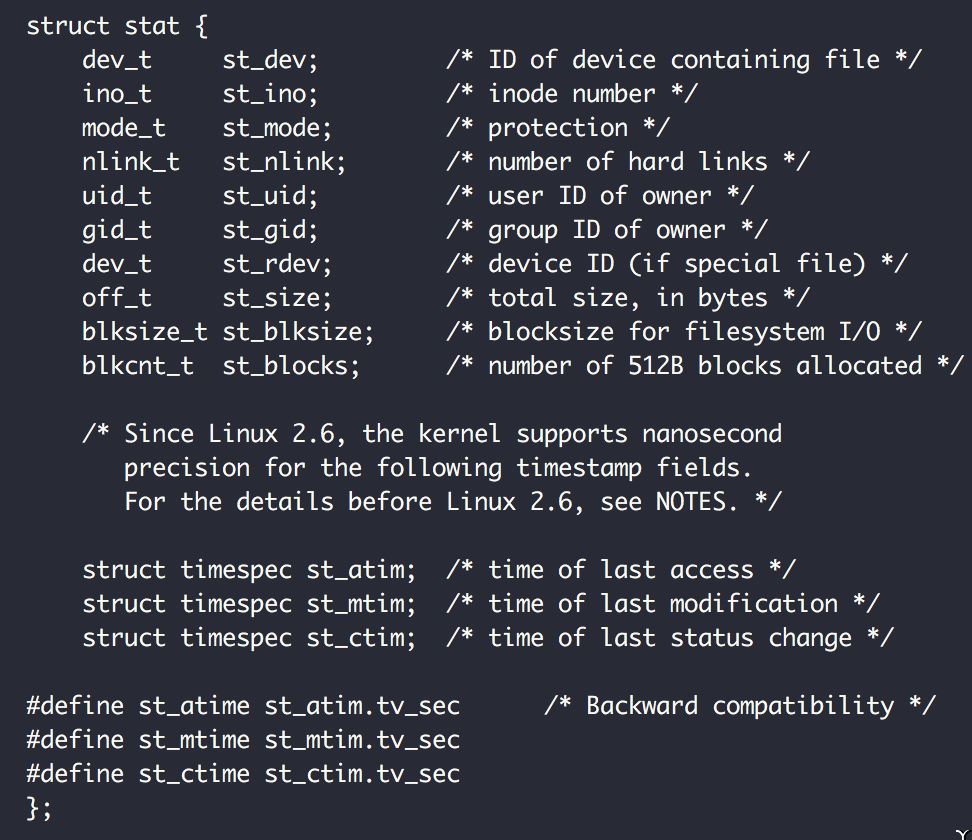
\includegraphics[width=0.6\textwidth]{./Figures/struct-stat.png}}
    \caption{struct stat 结构体}
    \label{fig:stat}
\end{figure}

这个包含了一个文件的所有属性信息, 充分的理解 Linux 中的文件属性将会有益于开发一个文件系统,
因为文件属性是所有文件操作的基石. 接下来将会解释这一结构体.

\fbox{st\_dev} 是文件所在的设备号, Linux 内核源码中的
\href{https://github.com/torvalds/linux/blob/master/Documentation/admin-guide/devices.txt}{devices.txt}
包含了所有已注册的设备号, 假如当前目录下面有一个 hello.c 文件, 使用 stat 命令查看其属性,
除了文件名称外, 其他均是 stat 结构体中的内容, 如下所示

\begin{lstlisting}[style=verb]
$ stat hello.c
  File: 'hello.c'
  Size: 8               Blocks: 8          IO Block: 4096   regular file
Device: 801h/2049d      Inode: 1054054     Links: 1
Access: (0664/-rw-rw-r--)  Uid: ( 1000/ xserver)   Gid: ( 1000/ xserver)
Access: 2018-09-14 21:05:50.295830427 +0800
Modify: 2018-09-14 21:05:50.295830427 +0800
Change: 2018-09-14 21:05:50.295830427 +0800
 Birth: -

$ df .
Filesystem     1K-blocks    Used Available Use% Mounted on
/dev/sda1       40636768 6056328  32493172  16% /

$ ls -hl /dev/sda1
brw-rw---- 1 root disk 8, 1 Sep 13 08:05 /dev/sda1
x
\end{lstlisting}

在显示的结果中,  size 对应用 \fbox{st\_size} 表示文件的大小, 单位为字节,
Blocks 指的就是物理磁盘块的个数, 而 IO Block 指的则是文件读写的块大小.
一般地, 磁盘和文件读写操作都是分块进行的, 一次操作一个块.
物理磁盘的块大小一般可以通过 lsblk -o NAME,PHY-Sec 来查看, 而 IO 块的大小通过上述
\fbox{stat} 即可查看. 假如一个磁盘的物理块大小为 512 字节, 那么一个 1 字节的文件也要至少
占用 512 字节的空间, 而若读写 IO 为 4096 字节, 则 1 字节的文件要至少要写一次, 即写入 4096
个字节, 占用 8 个物理磁盘块. 这个文件的设备号的值为 801h/2049d, 前面一个数值是 16 进制,
后一个是十进制值, 十六进制中, 第一个数字表示主设备号, 剩下两位表示从设备号, 这个可以从上述
命令的后两个命令得以验证. \fbox{st\_ino} 表示文件的 inode 节点索引,
inode 节点本身是一个数据结构, 其具体定义可以在
\href{https://github.com/torvalds/linux/blob/master/include/linux/fs.h}{fs.h} 中查看.
它包含了 st\_buf 中所有的信息以及附加的许多其他额外信息, 在 Linux 中, 区别文件的唯一标志是
inode 编号, 而非文件名称, 可以通过 inode 节点值删除特殊名称的文件,
\fbox{find /path/to/file/dir -inum [inode-number] -exec rm -i {} \;}. 接着是 Links,
它表示了指向该文件的硬链接数目, stat 中对应的字段为 \fbox{st\_nlink}.
\fbox{st\_uid, st\_gid} 分别表示用户 ID 和组 ID, 如果文件是字符设备,
则 \fbox{st\_rdev} 表示字符设备的 ID. 最后是 \fbox{st\_mode},
这个字段由文件类型和文件权限组合而成, 使用如下宏可以判断一个文件的类型
\begin{lstlisting}[style=verb]
S_ISLNK(mode)
S_ISREG(mode)
S_ISDIR(mode)
S_ISCHR(mode)
S_ISBLK(mode)
S_ISFIFO(mode)
S_ISSOCK(mode)
\end{lstlisting}
而使用如下值与 st\_mode 进行与操作, 可以判断文件的权限
\begin{lstlisting}[style=verb]
mode & S_IWUSR
mode & S_IXUSR
mode & S_IRGRP
mode & S_IWGRP
mode & S_IXGRP
mode & S_IROTH
mode & S_IWOTH
mode & S_IXOTH
\end{lstlisting}

另外的一个函数是 truncate, 除非是实现一个只读文件系统, 否则该函数也是必须要实现的,
因为写一个文件, 首先要执行 truncate 函数对文件进行扩大或者缩小.

对于其他函数, 可自行查看 fuse 源码中的注释, 限于篇幅, 此处不一一介绍.

\subsection{FUSE 调试开发}
fuse 的一些重要选项如下:
\begin{itemize}
    \item -d : 启用调试输出
    \item -f: 以前台模式运行, 方便调试, 此时 fuse 的工作目录是你启动客户端所在的目录,
        没有 -f 时, 工作目录是切换到 \fbox{/}, 因此, 务必使用绝对路径.
    \item -s: 以单线程运行, 方便调试.
\end{itemize}

调试时务必启用 \fbox{-f} 选项, 否则 fuse 会断开 stdout 和 stderr 的连接,
此时 printf 和 fprintf 将失效, 一个较好的方式是将文件的日志写到一个日志文件中去.

\subsection{基于 BBFS 寻找接口切入点}
\label{sec:rlfsentry}

BBFS 系统实现了几乎所有 FUSE 提供的接口, 大多数是直接调用 linux 系统里对应的系统 API 完成
. 在 BBFS 源码之上, 添加调试信息, 观察不同操作对应的具体函数流调用. 首先编译 BBFS 系统:

\begin{lstlisting}[style=verb]
FUSEROOT=$HOME/fuse
wget http://www.cs.nmsu.edu/~pfeiffer/fuse-tutorial.tgz -O $FUSEROOT/fuse-tutorial.tgz
cd $FUSEROOT && tar zxvf fuse-tutorial.tgz
cd fuse-tutorial-2018-02-04
./configure
make
\end{lstlisting}

注意, 可能需要配置 libfuse 环境.完成编译后, 生成的可执行文件位于 src 目录, 不需要额外进行安装.
使用方法:

\begin{lstlisting}[style=verb]
# 挂载到 ~/point 目录下
 ./bbfs -o nonempty . ~/point/
# 卸载
fusermount -u ~/point
\end{lstlisting}

在 bbfs 源码中各个函数入口开始处, 添加调试信息, 测试不同操作, 打印函数流
\begin{lstlisting}[style=verb]
# 写入文件操作

$ dd if=/dev/zero of=a.iso bs=4097 count=1

[+] <Fri Aug 31 17:01:37 2018>|<bb_open>#271
[+] <Fri Aug 31 17:01:37 2018>|<bb_getxattr>#519
[+] <Fri Aug 31 17:01:37 2018>|<bb_truncate>#234
[+] <Fri Aug 31 17:01:37 2018>|<bb_getattr>#37
[+] <Fri Aug 31 17:01:37 2018>|<bb_flush>#438
[+] <Fri Aug 31 17:01:37 2018>|<bb_getxattr>#519
[+] <Fri Aug 31 17:01:37 2018>|<bb_write>#338
[+] <Fri Aug 31 17:01:37 2018>|<bb_write>#375
[+] <Fri Aug 31 17:01:37 2018>|<bb_write>#378
[+] <Fri Aug 31 17:01:37 2018>|<bb_write>#338
[+] <Fri Aug 31 17:01:37 2018>|<bb_write>#375
[+] <Fri Aug 31 17:01:37 2018>|<bb_write>#378
[+] <Fri Aug 31 17:01:37 2018>|<bb_flush>#438
[+] <Fri Aug 31 17:01:37 2018>|<bb_release>#463
\end{lstlisting}

将文件写到挂载目录时,发生了如下主要事件:
在 open 中打开文件, 在 write 中写文件内容,
每个块的最大尺寸为 4KB(4096 Bytes), 比如上述生成 4097 KB
的块, 将会分成两次操作, 第一次写 4KB, 第二次写 1 Byte.
所有操作在写完后, 将会调用 flush 刷新缓存, 最后调用 release 关闭文件.

\begin{lstlisting}[style=verb]
# 显示文件列表

$ ls -l

[+] <Wed Aug 29 11:35:51 2018>|<bb_opendir>#581
[+] <Wed Aug 29 11:35:51 2018>|<bb_getattr>#75
[+] <Wed Aug 29 11:35:51 2018>|<bb_readdir>#629
[+] <Wed Aug 29 11:35:51 2018>|<bb_getattr>#75
[+] <Wed Aug 29 11:35:51 2018>|<bb_getxattr>#517
[+] <Wed Aug 29 11:35:51 2018>|<bb_getattr>#75
[+] <Wed Aug 29 11:35:51 2018>|<bb_releasedir>#673
\end{lstlisting}

读取文件属性时基本上是 opendir, readdir, getattr, getxattr, releasedir 这几个操作.

用类似的方法, 结合其他的观察以及调试, 可以得知, fuse 在启动后, 会使用 init 函数来进行初始化
, 我们可以在这一步去存储节点上并行的将文件取回来; 当文件写完或者访问后, fuse 会调用 relase 函数,
所以当用户执行完写操作后, 我们判定为写操作后, 便可将文件并行的发送到服务器存储节点上.

所以 init 函数和 release 函数是我们设计 RLFS 系统的切入点.

\section{RLFS 系统设计}
\subsection{系统概览}
在 \ref{sec:rlfsentry} 中我们提到了 RLFS  系统的切入点, 所以 RLFS 系统的大致框架如图
\ref{fig:rlfs} 所示.

\begin{figure}[H]
    \centerline{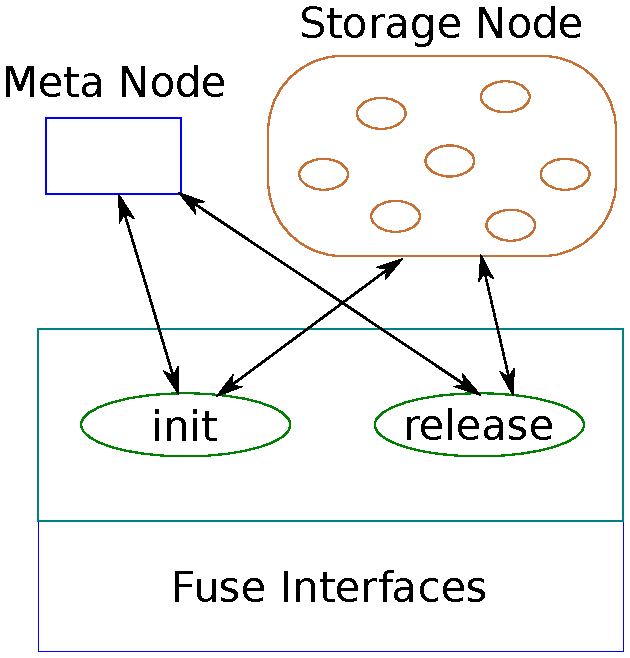
\includegraphics[width=0.5\textwidth]{./Figures/rlfs.pdf}}
    \caption{RLFS 基本结构}
    \label{fig:rlfs}
\end{figure}

当我们在 release 里面检测到写操作完毕后, 我们将会将写入的数据分块, 并并行发送到存储节点
(Storage Node), 每发送一个文件块, 将会把块信息(如位于哪一个存储节点, 块的序列值等信息)
发送到元数据服务器(Meta Node) 上, 当用户重新挂载时, RLFS 将会在 init 函数中远程查询元数据服
务器, 并从存储节点上取回文件块到本地, 合成一个完整的文件, 呈献给用户.
整个系统的工程结构如下

\begin{lstlisting}[style=verb]
├── CMakeLists.txt*
├── README.md
├── bbfs/
├── scripts/
│   ├── fuse2env*
│   ├── install-deps.sh*
│   ├── install-rlfs.sh*
│   ├── nodeconfig*
│   ├── plotperf.py
│   └── tarme.sh*
└── src/
    ├── include/
    │   ├── rlfs.h
    │   ├── rlfsop.hpp
    │   └── util.hpp
    ├── rlfsc.c
    └── rlfsd.c
\end{lstlisting}

整个工程采用 cmake 构建, 项目规模约 2k 行 C 代码(含注释).

简要介绍一下各个目录和文件:
\fbox{bbfs/} 目录为 BBFS 系统的代码, 其中剔除了 RLFS 系统实现的 FUSE 接口.

\fbox{scripts/} 目录为工具脚本和配置文件目录, 其中 \fbox{fuse2env} 用于激活 fuse 开发环境,
\fbox{install-rlfs.sh} 用于无痛安装 rlfs 系统, \fbox{tarme.sh} 用于打包项目为 .tgz 文件,
\fbox{plotperf.py} 用于绘画测试图.

\fbox{src/} 目录为 RLFS 源码目, 其中 \fbox{include/} 下包含了所有用到的头文件,
\fbox{rlfsc.c} 为客户端代码, \fbox{rlfsd.c} 为服务器端代码.


\subsection{数据结构}

为了使得服务器端和客户端能够进行一致的交互, 双方必须约定好一些规则, 下面是 RLFS 系统用到的
一些数据结构, 环境变量等.

\subsubsection{文件块容量}
默认块容量为 4 MB, 服务器端和客户端必须大小一致, 编译时必须同时生成客户端和服务器端,
块容量值无法动态更改, 只能在编译时指定.

\subsubsection{系统目录}

客户端和服务器端上均可以设置一个环境变量 \fbox{RLFSROOT} 作为 RLFS 系统的根目录, 如果没有设置,
则设置 RLFSROOT 为 \verb|$HOME| 的值. RLFS 在客户端和服务器端上用的目录如下:

\begin{itemize}
    \item 客户端缓存目录: \verb|$RLFSROOT/.rlfs|
    \item 元数据服务器端的元数据目录: \verb|$RLFSROOT/rlfsmeta|.
        该目录下一个文件对应一个元数据, 后缀为 \verb|.meta|.
        假如文件名称为 hello.iso, 那么则对应的有一个 hello.iso.meta 文件.
\end{itemize}


\subsubsection{元数据文件格式}
元数据文件为一个二进制文件, 其结构如图 \ref{fig:filemeta} 所示.

\begin{figure}[H]
    \centerline{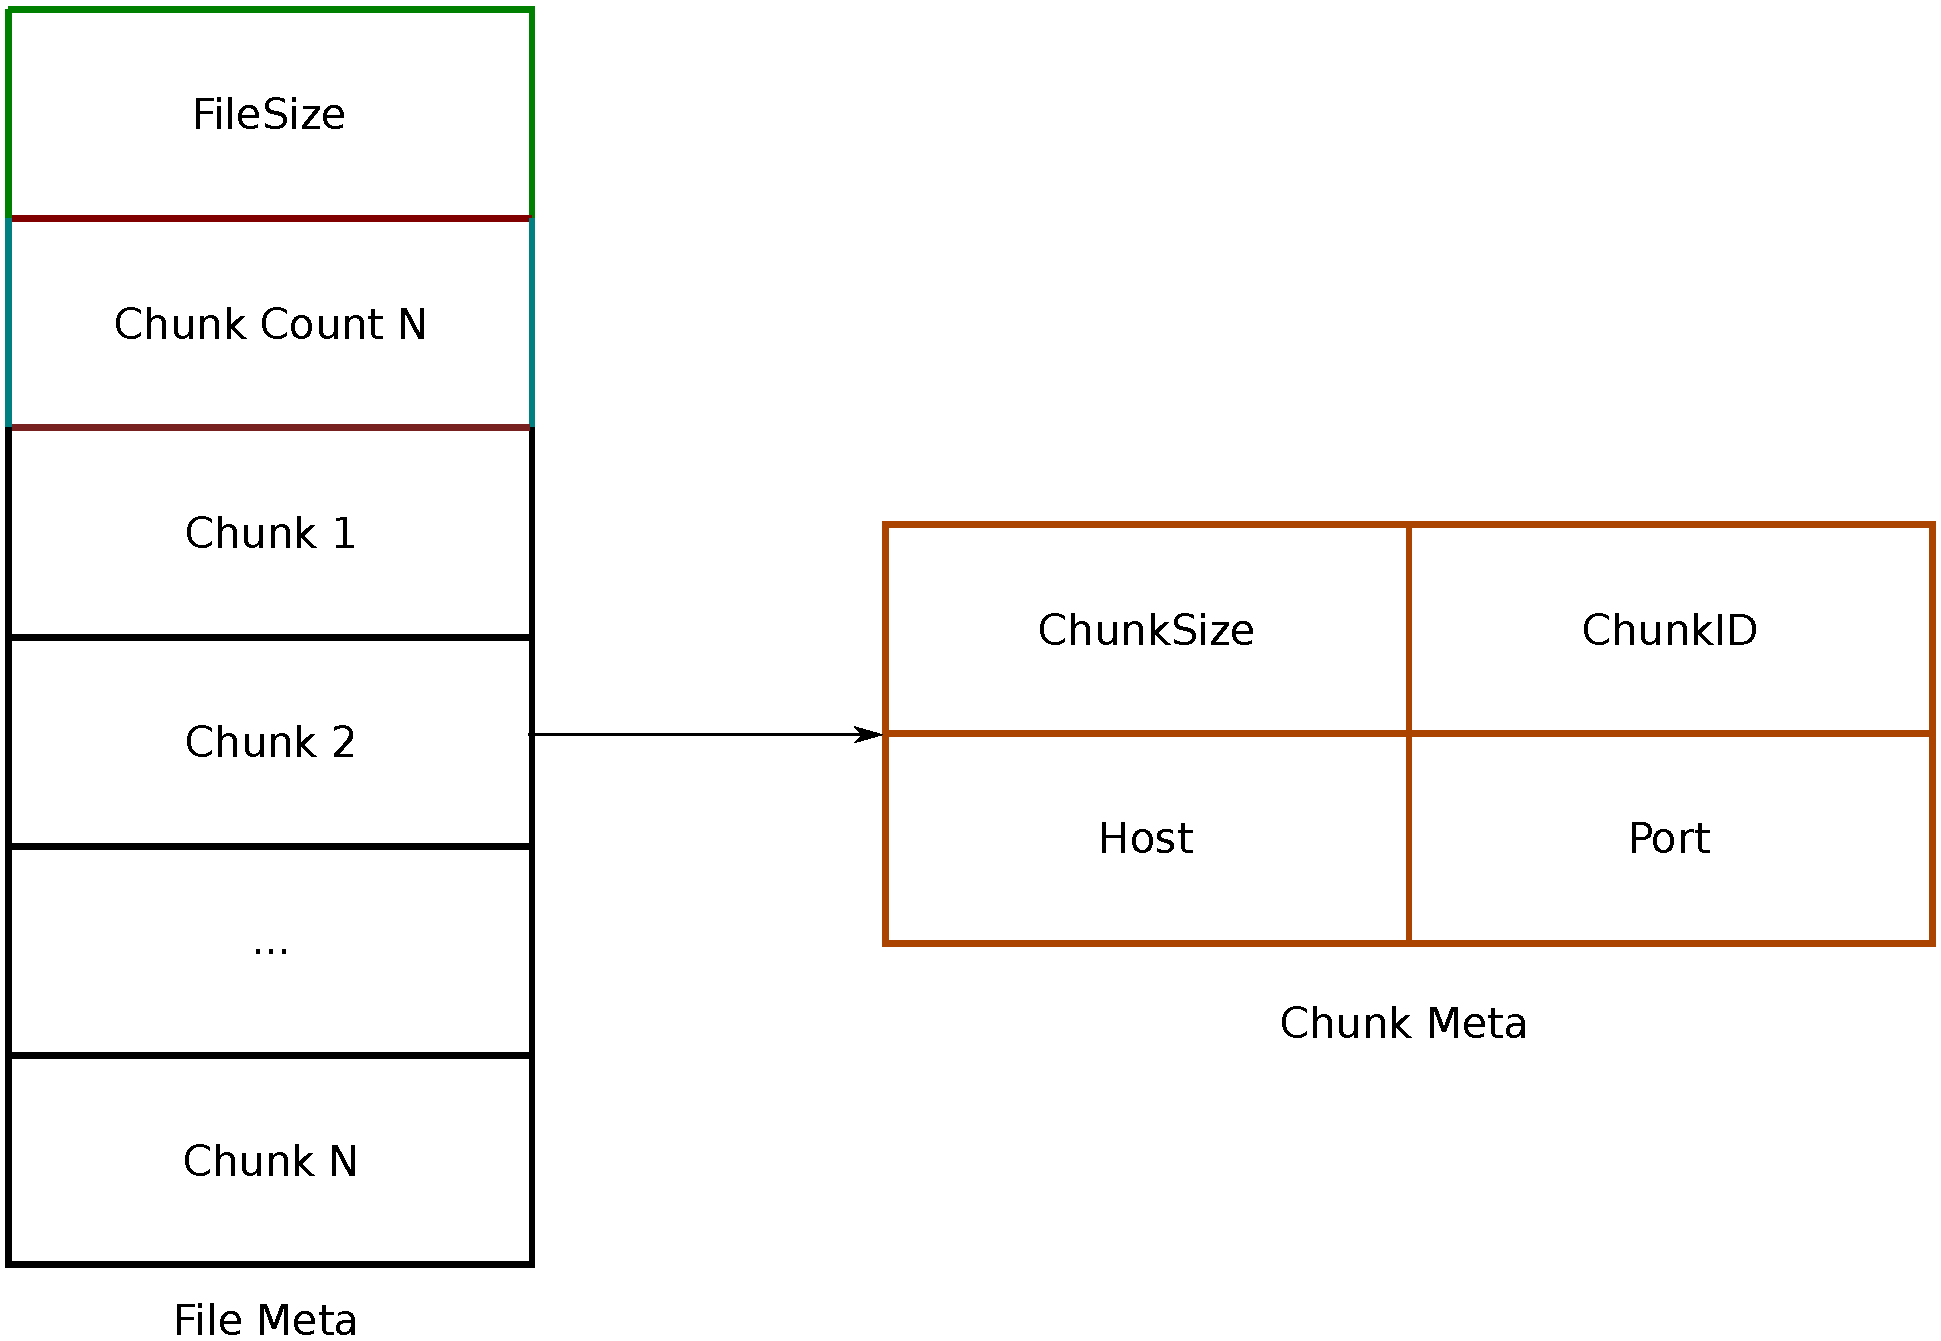
\includegraphics[width=0.7\textwidth]{./Figures/filemeta.pdf}}
    \caption{文件元数据结构}
    \label{fig:filemeta}
\end{figure}

文件元数据(File Meta)依次存放着文件大小(filesize),文件块数目N(chunknum), 文件块记录(chunkmeta).
filesize 的类型为 long, chunknum 的类型为 unsigned.

在文件块元数据(Chunk Meta) 中, ChunkSize 是文件块的实际大小(不是块容量 \verb|FILE_CHUNK|),
ChunkID 是该块在文件中的序列值.文件在发送到存储节点时, 每次发送一个块容量大小的文件块,
当文件剩余内容不足块容量时, 发送实际剩余大小的内容,
所以如果文件的各个块中, 只有最后一块可能小于块容量大小, 其他均等于块容量.
除此之外也包含了文件块所在节点的地址(Host)和连接端口(Port).

\subsubsection{通信协议}
目前, 通信端口为 3490, 通信协议的结构如图 \ref{fig:rlfsmsg} 所示.

\begin{figure}[H]
    \centerline{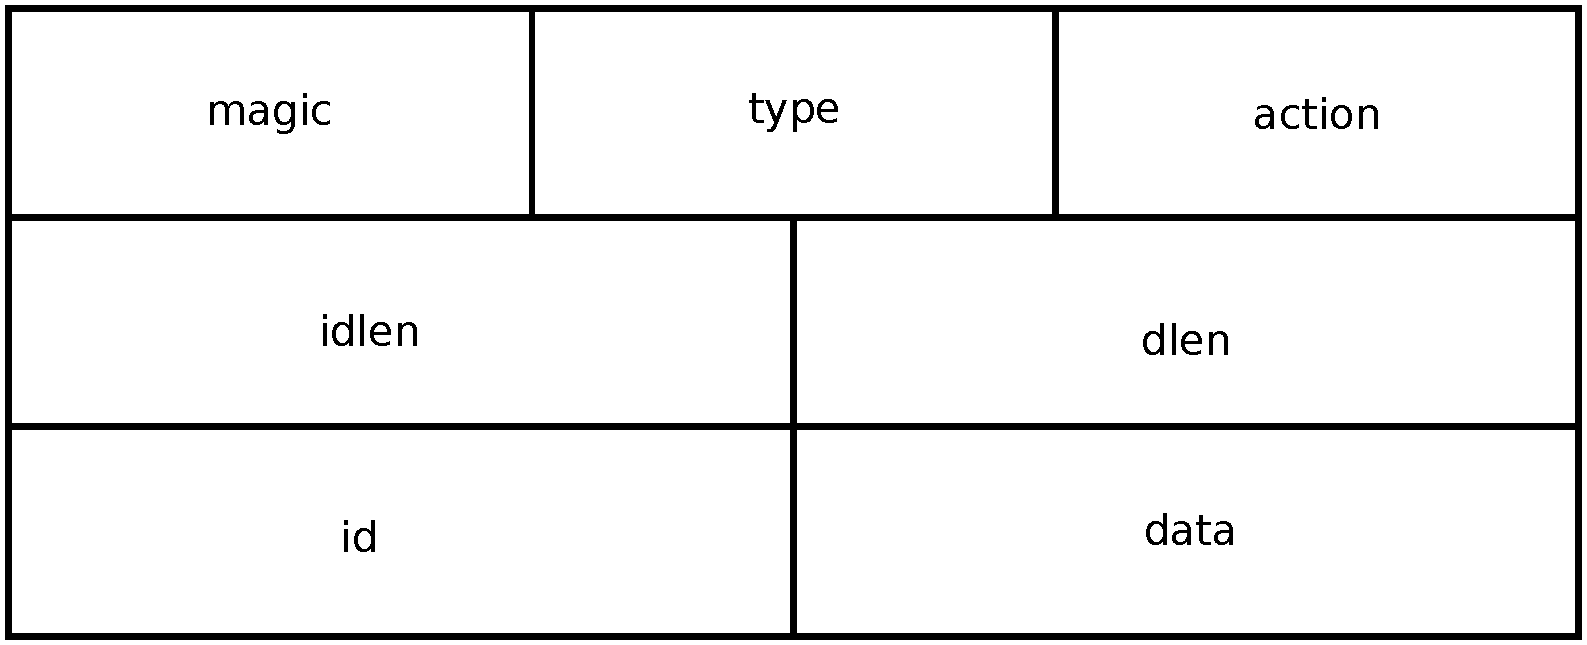
\includegraphics[width=0.7\textwidth]{./Figures/rlfsmsg.pdf}}
    \caption{通信协议结构}
    \label{fig:rlfsmsg}
\end{figure}

magic 恒定为 \fbox{RLFS}, 如果为 \fbox{TEST} 则说明这这是一个测试消息, 服务器端将不做任何反馈,
直接丢弃. 消息类型(type)有如下几种:

\begin{itemize}
    \item MSG\_FILEMETA: 处理文件元数据
    \item MSG\_CHUNKDATA: 处理文件块数据
\end{itemize}

对应不同的消息有不同的动作(action)

\begin{itemize}
    \item ACTION\_META\_CREATE: 创建元数据文件
    \item ACTION\_META\_FILL: 填充元数据文件
    \item ACTION\_META\_FETCH: 获取元数据文件
    \item ACTION\_CHUNK\_STORE: 存储文件块
    \item ACTION\_CHUNK\_FETCH: 获取文件块
\end{itemize}

\section{系统评估}
测试系统均为 Ubuntu 16.04 x64, 至少 500MB RAM.
生成 8MB, 64MB, 128MB, 256MB 的四个测试文件(内容随机填充), 命令如下:

\begin{lstlisting}[style=verb]
declare -A iso=(["8"]=2048 ["64"]=16348 ["128"]=32768 ["256"]=65536)
for i in ${!iso[@]}
do
    dd if=/dev/urandom of=${i}MB.iso bs=4k count=${iso[${i}]} &> /dev/null
    md5sum ${i}MB.iso
done
\end{lstlisting}

本例中用的四个文件名称以及 md5 值如下
\begin{lstlisting}[style=verb]
737e2f20e584081b9ab7531cbcab06e3  256MB.iso
c2de13928f423109f83693d05167c03b  64MB.iso
5268b40a56d3d9ad83e7c148d088a0aa  8MB.iso
eee056218803a7187c906a1921d92b08  128MB.iso
\end{lstlisting}

测试过程中, 在各个节点上运行 \fbox{rlfsd} 服务端, 配置节点文件,
在客户端上运行 \fbox{rlfsc}, 启动后, 拷贝四个 iso 文件到挂载目录, 等待操作完毕后,
关闭 \fbox{rlfsc}, 将本地缓存目录 \$RLFSROOT/.rlfs 中的四个 iso 文件删除,
再次运行 \fbox{rlfsc}, rlfsc 将会自动连接元数据服务器并并发取回四个文件后, 待文件取回后,
检验文件 md5 值, md5 值一致则说明文件传输一切正常. 数据发送和接收过程中,
会记录每一个数据块的发送或者接收时间.

\subsection{RLFS 系统的安装与运行}

在 Ubuntu 16.04 x64 系统上课以执行项目中的 \fbox{rlfs-install.sh} 脚本自动安装依赖, 自动配
置环境, 自动安装 RLFS 系统到 \fbox{\$HOME/.local/rlfs} 中, 安装完成后可以在任意目录执行
\fbox{rlfsc}, \fbox{rlfsd} 命令. 其他系统, 则需要自行配置依赖, 依赖包括 libfuse 2.9.x,
OpenSSL 1.1.x, cmake 3.12+, gettext, libtool,  pkg-config 等.

单独一个 rlfsc 命令执行后, 显示如图 \ref{fig:rlfsc-help} 所示.

\begin{figure}[H]
    \centerline{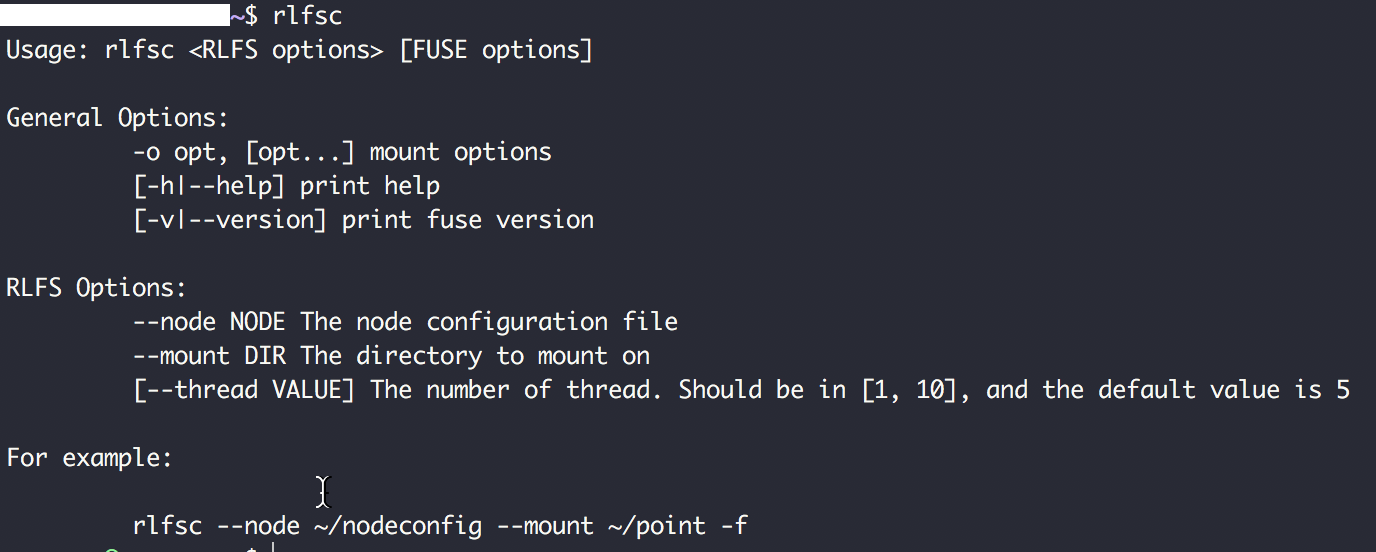
\includegraphics[width=1.0\textwidth]{./Figures/rlfsc-help.png}}
    \caption{rlfsc 帮助界面}
    \label{fig:rlfsc-help}
\end{figure}

RLFS 提供的选项有三个, \fbox{\Verb|--node|} 用于指定节点配置文件, 节点配置文件的格式十分简单,
一个节点占据一行, 写入节点的 IP 地址和端口号(以空格隔开), 以 `\#' 号开头的行将被视作注释行,
样例配置如下

\begin{lstlisting}[style=verb]
# The virutual machine
192.168.56.6 3490
# A
#192.168.200.42 3490
# B
#192.168.200.43 3490
# C
#192.168.200.44 3490
# D
#192.168.200.45 3490
\end{lstlisting}

\fbox{\Verb|--mount|} 用于指定挂载目录, 请确保该目录存在. \fbox{\Verb|--thread|} 用于指定
线程数, 线程数的值应该为一个整数, 最小为 1, 最大为 10, 默认为 5, 一般可以忽略.

\subsection{数据测试}
由于机器不充足, 分布式节点只用了四台, 图 \ref{fig:rlfs-startup} 是一个运行示意图.

\begin{figure}[H]
    \centerline{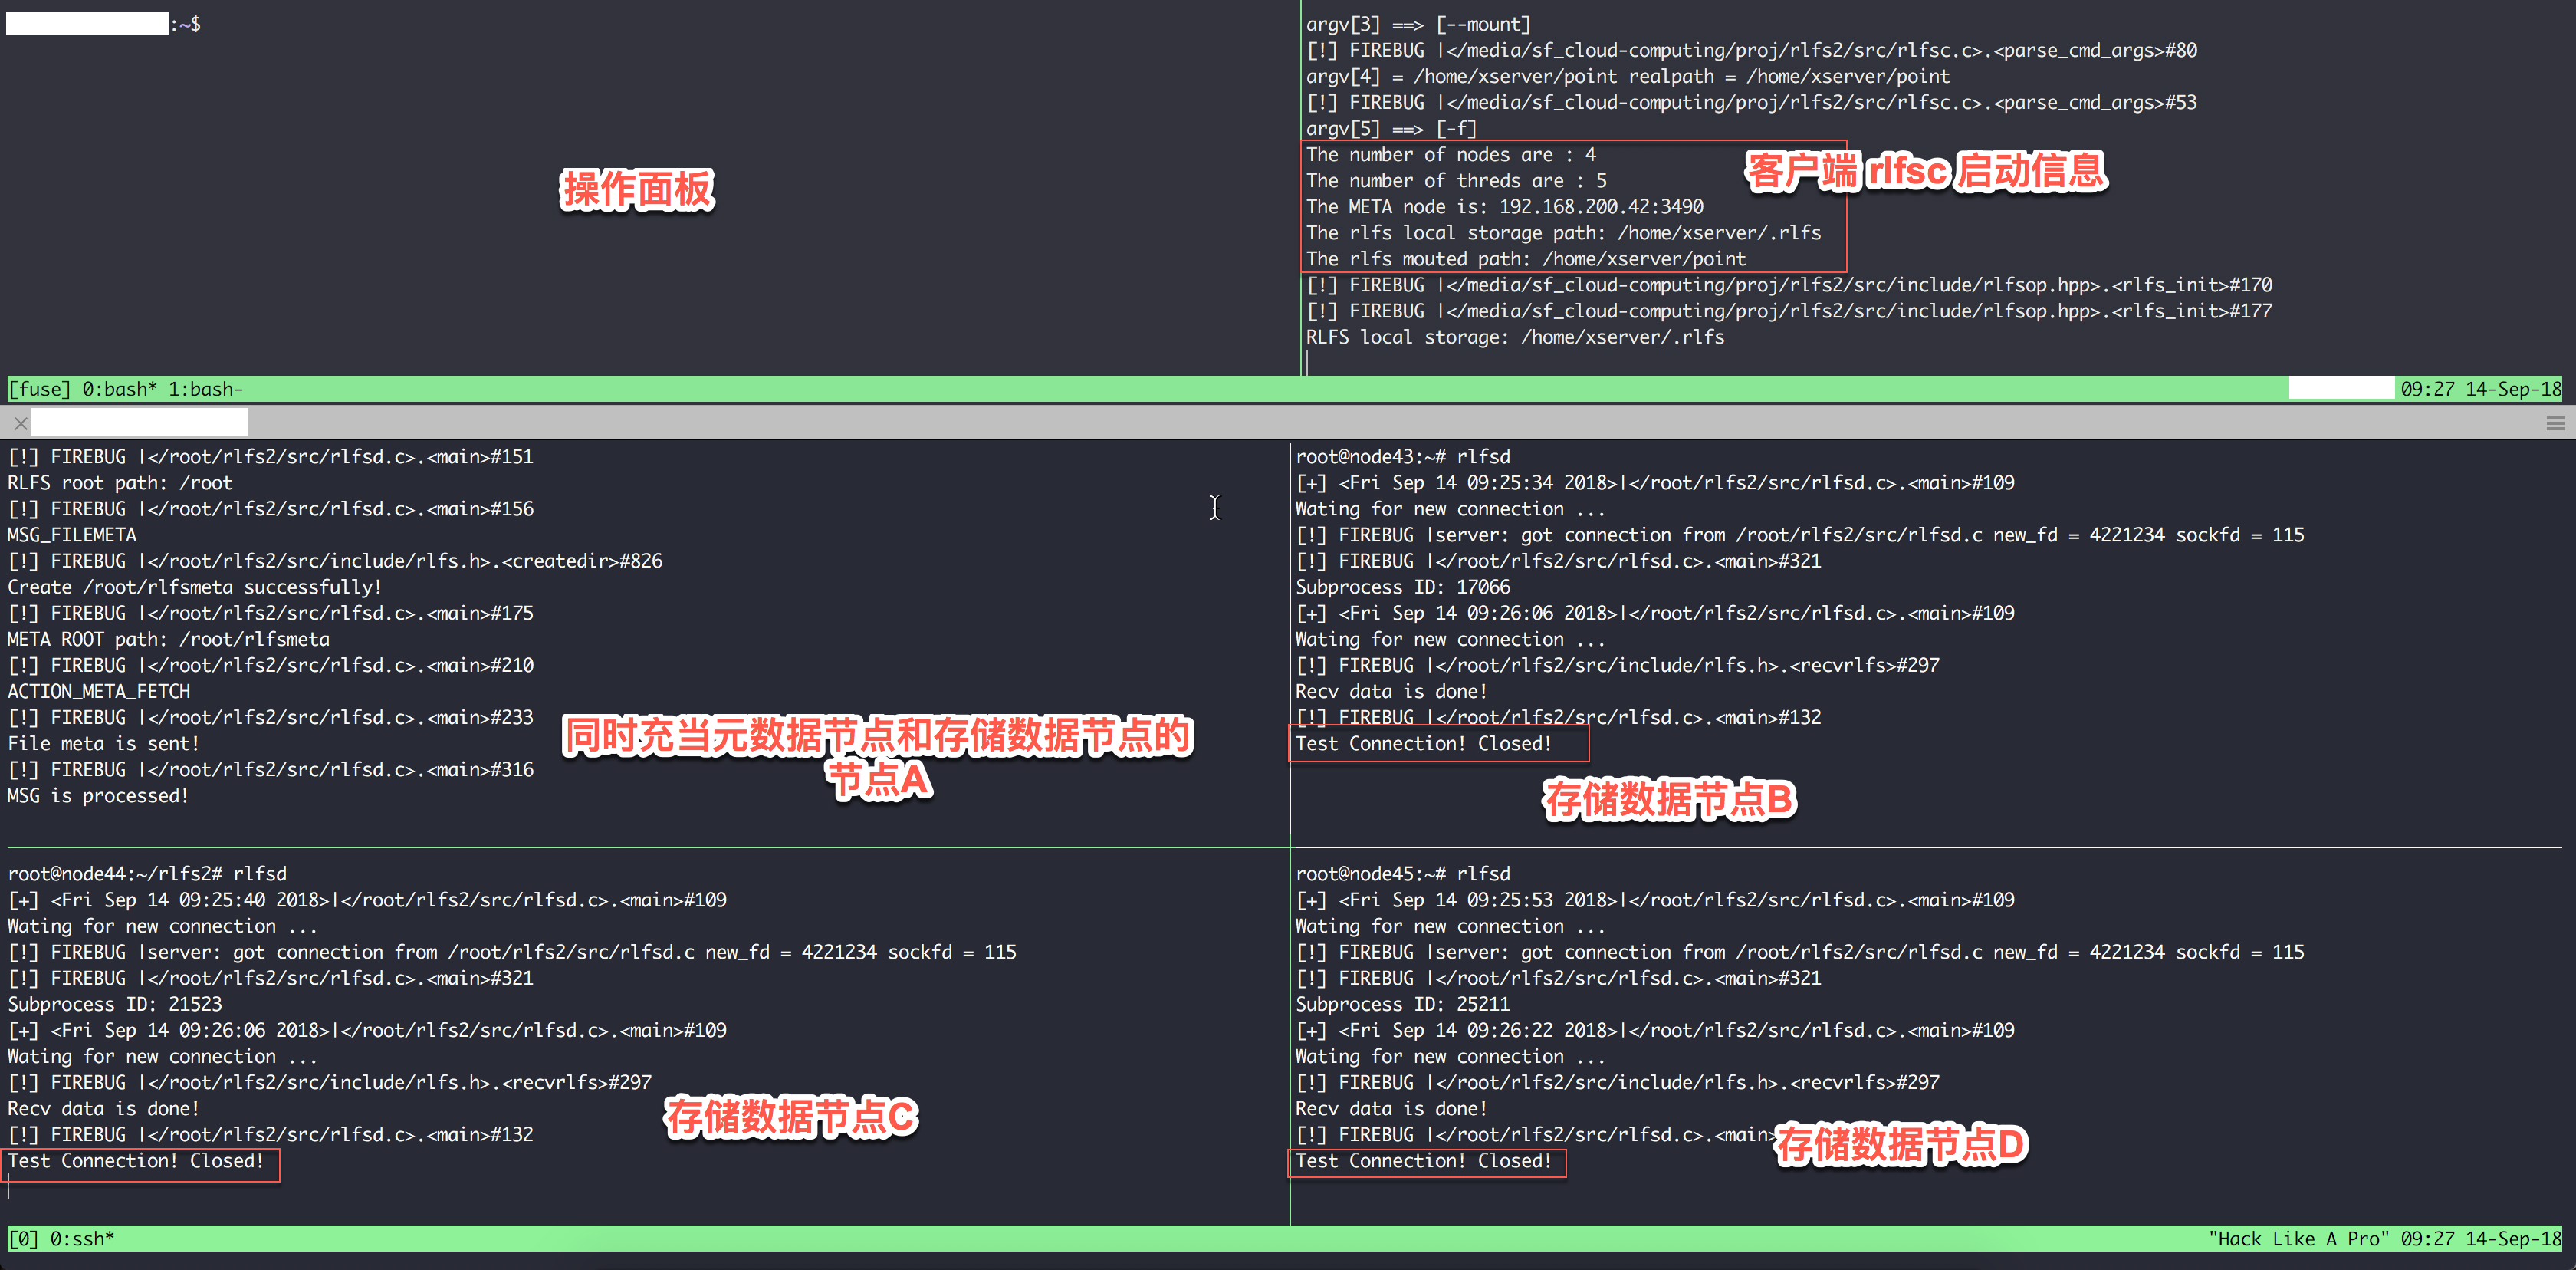
\includegraphics[width=1.0\textwidth]{./Figures/startup.png}}
    \caption{RLFS 启动示意图}
    \label{fig:rlfs-startup}
\end{figure}

rlfsc 启动后, 会显示线程数, 节点数, 元数据服务器的地址和端口, RLFS 缓存目录以及挂在目录等信
息, 首次启动会发送 \fbox{TEST} 消息来测试有多少节点存活. 图 \ref{fig:rlfs-startup} 中使用了
四个节点, 其中节点 A 同时充当元数据服务器和存储数据服务器, 其他节点 B, C, D 均为存储数据节
点. 从存储节点获取数据块的示意如图 \ref{fig:fetchchunk} 所示.

\begin{figure}[H]
    \centerline{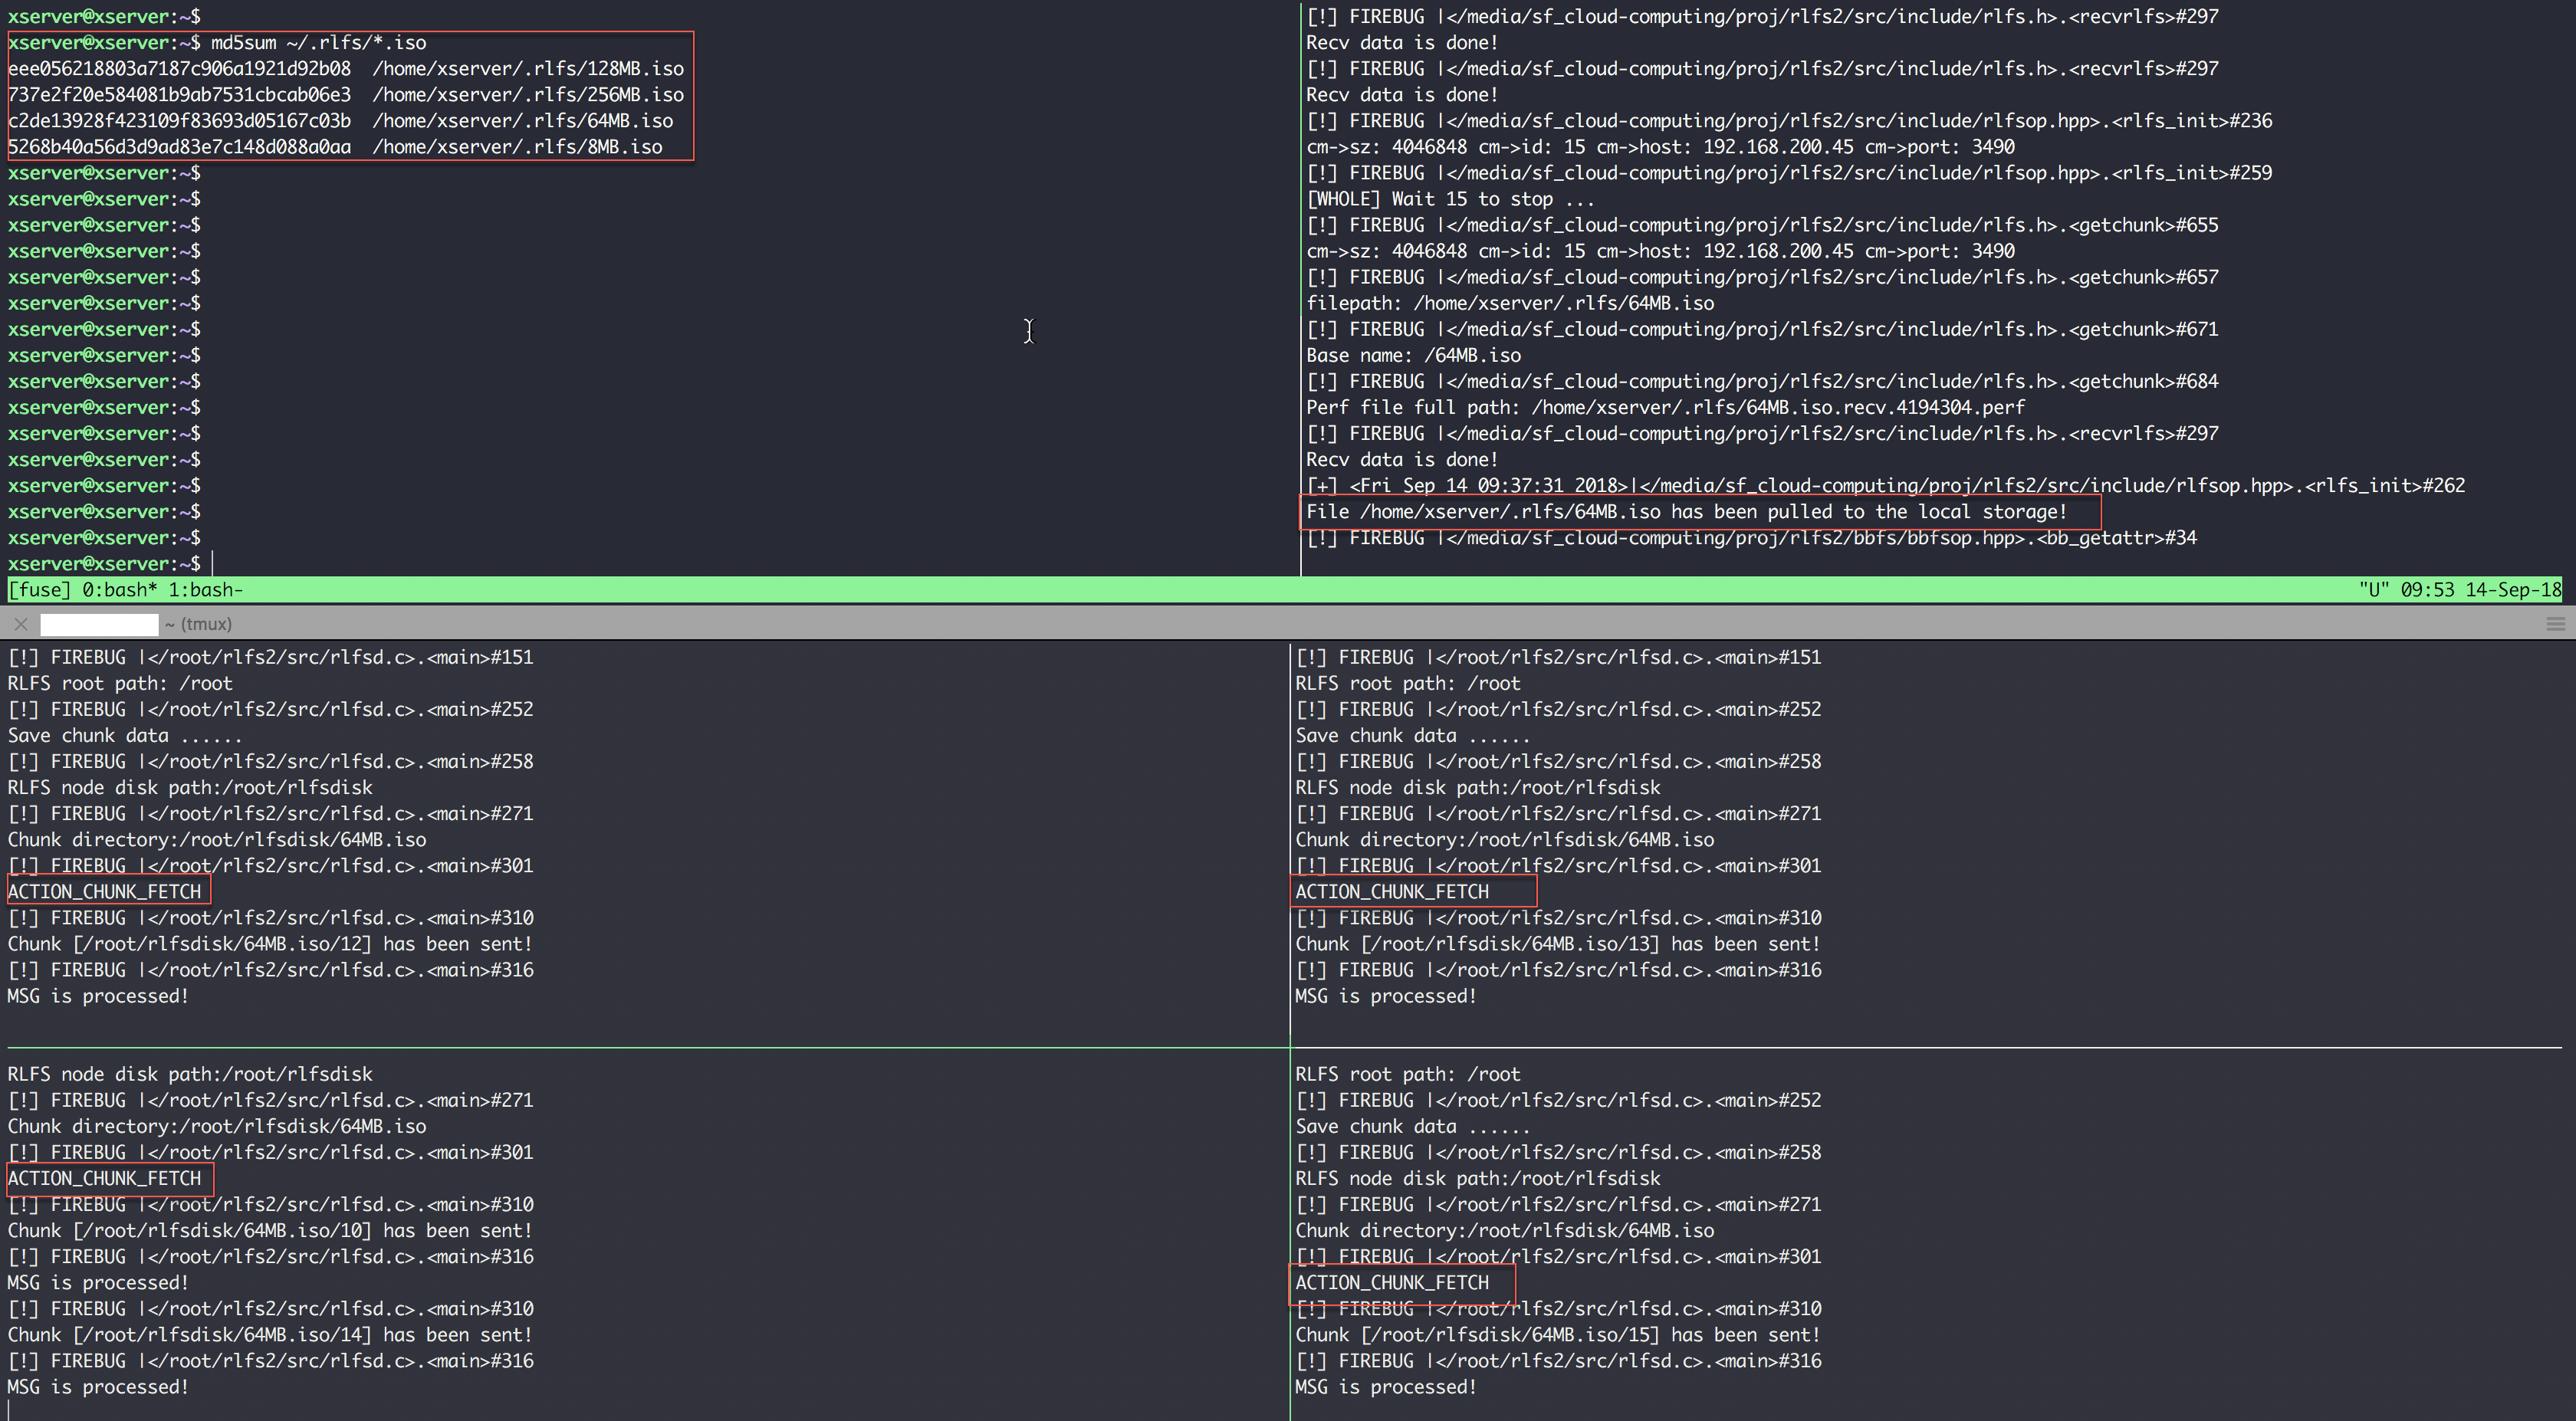
\includegraphics[width=1.0\textwidth]{./Figures/fetchchunk.png}}
    \caption{从数据节点取回文件}
    \label{fig:fetchchunk}
\end{figure}

为了对数据传输进行测试, 将文件块的发送开始和结束时间戳依次记录在一个二进制文件中,
如果一个文件有 N 个文件块, 那么将具有 N 个记录, 每个记录包含了处理该文件块的始末时间戳.

对一台机器进行测试, 该机器同时充当元数据服务器和存储数据服务器,
其结果如图 \ref{fig:onenode} 所示.

\begin{figure}[H]
    \centerline{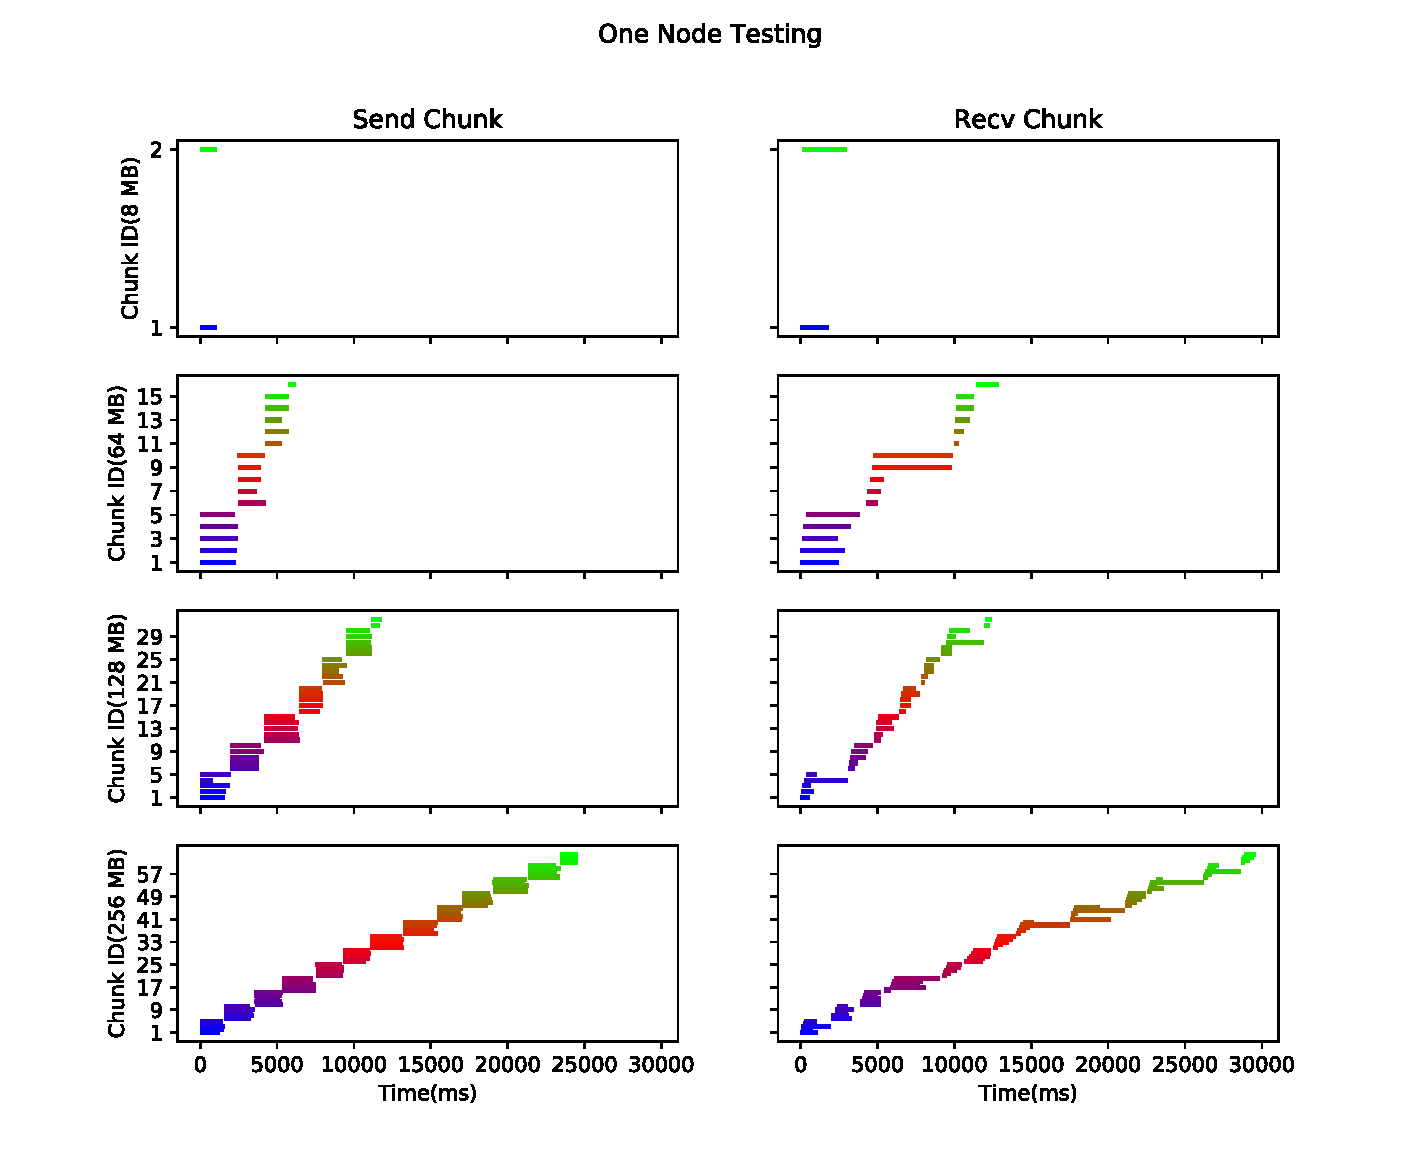
\includegraphics[width=1.0\textwidth]{./Figures/onenode.pdf}}
    \caption{一个节点测试}
    \label{fig:onenode}
\end{figure}

以图 \ref{fig:onenode} 为例进行说明, 图一共 4 行 2 列, 左侧列对应于发数据, 右侧对应于收数据,
每一行对应一个测试文件, 比如第一行对应的为 8MB 的文件, 每个子图的 Y 轴为文件块的序列值
(Chunk ID), 因为 RLFS 中默认块的大小为 4 MB, 所以 8MB 的文件只有两个文件块, 即发送两次,
测试时用的线程数为默认线程数 5, 子图的 X 轴为时间, 单位为毫秒.
四个节点测试的结果如图 \ref{fig:fournodes} 所示.

\begin{figure}[H]
    \centerline{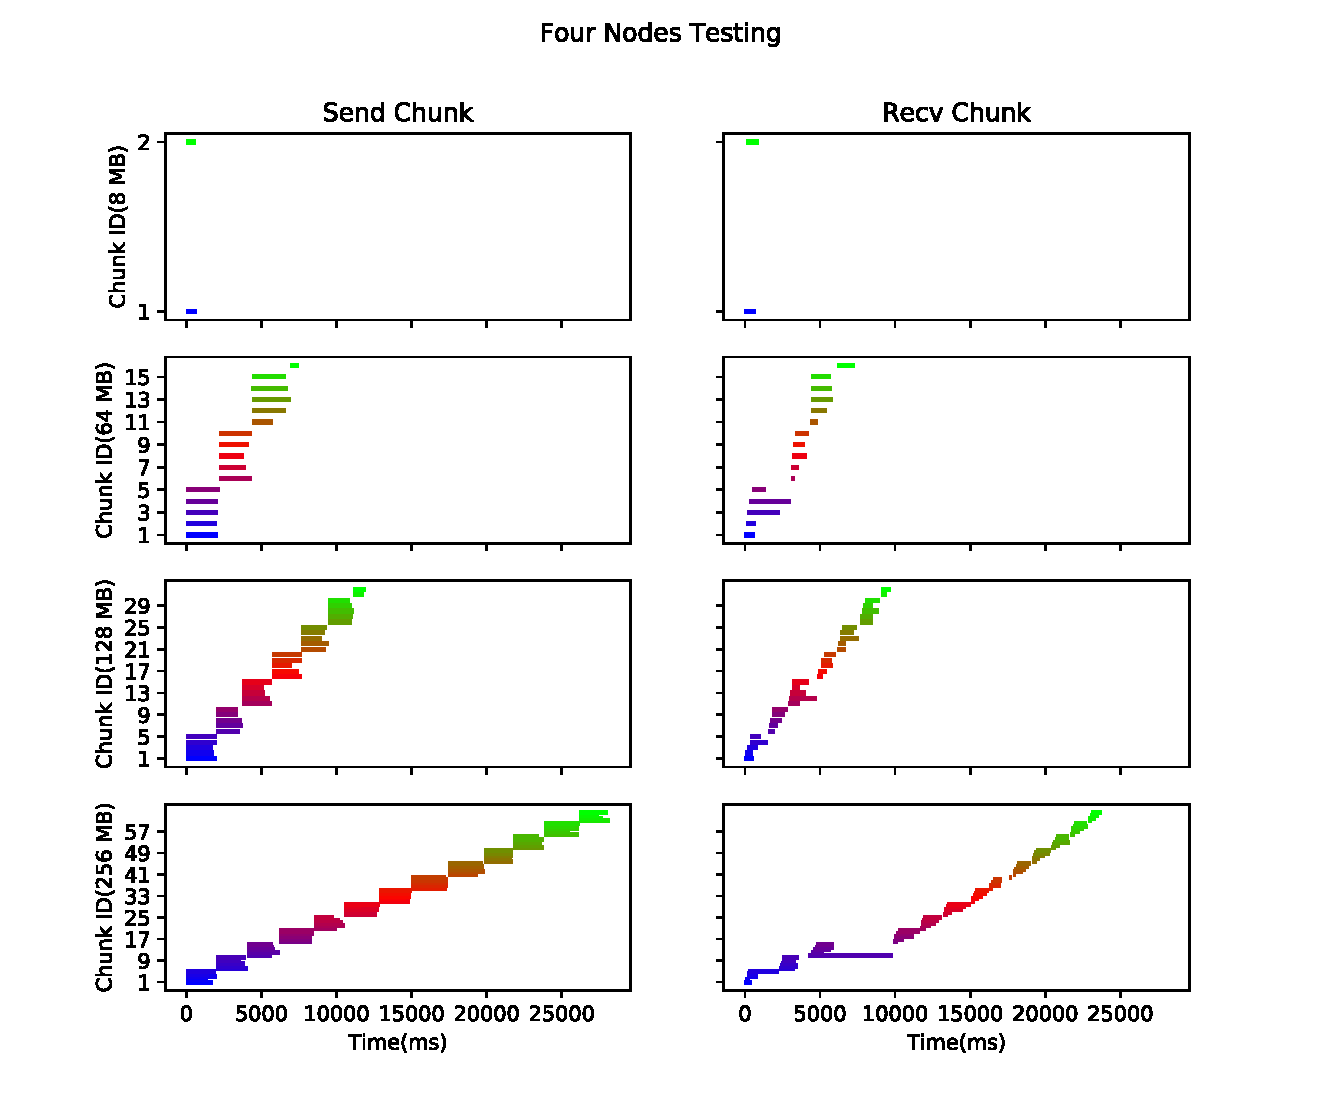
\includegraphics[width=1.0\textwidth]{./Figures/fournodes.pdf}}
    \caption{四个节点测试}
    \label{fig:fournodes}
\end{figure}

和单节点相比, 多节点传输在发送数据上并不占据优势, 但是在收数据上却占有较为明显的优势.
这里也能明显的看到有的文件块占用的传输时间较长, 大大拖延了整体传输时间,
这是 RLFS 为了优化内存的使用, 启用的线程数一旦达到设定的线程数,
RLFS 将会停止启动新的线程, 而是等待所有的线程结束后,
线程释放内存后才继续启动新的线程进行文件传输. 这个可以再进一步优化,
比如设置一个完成任务的线程数占据总线程数的百分比阈值,
如果超过该阈值, 将自动启动新的线程发送数据, 这样将会减缓某些文件块传输拖延整个文件传输的进
度, 但是该优化暂时未在 RLFS 中实现.

\section{代码编码规范}
\subsection{命名}
所有结构体, 枚举值, 变量, 函数名均为小写, 当名称的长度超过 10 个字符时,
一律以下划线间隔, 小于 10 个字符时则在保证语义清晰的情况下连写.
宏的名称应该全部大写, 且以下划线分隔.

\subsection{行长度}
每行的长度的最多不应该超过 90.

\subsection{头文件包含}
头文件包含依次为语言级别的头文件, 系统级别的头文件, 第三方库头文件, 自定义头文件.
各个头文件的名称要按字母序增序排列.

\subsection{其他}
一般地一行一句代码, 但是当初始化变量时或者释放内存时,
在不至于行太长的情况下, 为方便代码理解, 可以多条语句写到一行上面. 如

\begin{lstlisting}[style=verb]

chunkmeta cm; memset(&cm, 0, sizeof(cm));

memcpy(chunkmsg->data + sizeof(cid), chunkdata, chunksz); free(chunkdata);

unsigned cid = *(unsigned *)parg; parg += sizeof(cid);

unsigned chunksz = *(unsigned *)parg; parg += sizeof(chunksz);
\end{lstlisting}

\section{参考}

\begin{enumerate}
    \item \href{https://beej.us/guide/bgnet/}{Beej's Guide to Network Programming Using Internet Sockets}
    \item \href{https://www.cs.nmsu.edu/~pfeiffer/fuse-tutorial/}{Writing a FUSE Filesystem: a Tutorial}
    \item \href{https://github.com/libfuse/sshfs}{A network filesystem client to connect to SSH servers}
    \item \href{https://en.wikipedia.org/wiki/Filesystem_in_Userspace}{Filesystem in Userspace} 
    \item \href{https://blog.csdn.net/juS3Ve/article/details/78237236}{吴锦华/明鑫: 用户态文件系统(FUSE)框架分析和实战} 
    \item \href{https://www.cs.hmc.edu/~geoff/classes/hmc.cs135.201109/homework/fuse/fuse_doc.html}{CS135 FUSE Documentation}
\end{enumerate}

\label{last_page_num}
\end{document}
